%% The following is a directive for TeXShop to indicate the main file
%%!TEX root = diss.tex

\chapter{Related Work}
\label{ch:RelatedWork}
In this chapter, we review the existing software and algorithms in the field of 3D computer vision. Section~\ref{sec:Toolbox} discusses the existing software and toolboxes for 3D computer vision. Section~\ref{sec:3DRecon_Tech} presents a comprehensive review of the field of image-based 3D reconstruction algorithms based on varied visual and geometric cues, which include \textit{stereo correspondence}, \textit{shading}, \textit{silhouette}, \textit{texture distortion}, and \textit{focus}.

\section{Toolboxes}
\label{sec:Toolbox}
There have been many attempts in developing computer vision or image processing frameworks that support rapid development of vision applications. There are multiple general vision libraries in this field including OpenCV~\cite{bradski2008learning}, VLFeat~\cite{vedaldi08vlfeat}, VXL~\cite{vxl17} and multiple Matlab libraries~\cite{KovesiMATLABCode, MariottiniPr_RAM05}. These libraries often provide tools for multiple image processing and computer vision problems, including low-vision tasks such as feature detection and matching, middle-level vision tasks such as segmentation and tracking, and high-level vision problems such as classification and recognition. All of these software frameworks and libraries provide vision components and algorithms without any context of how and when they should be applied. As a result, they often require expert vision knowledge for effective use. For example, many feature detectors and descriptors are provided by OpenCV but with no indication of under what conditions each works most effectively.

We have witnessed many successful software in the field of image-based reconstruction, which is a sub-field of 3D reconstruction. One of the most widely used open source software is PMVS developed by Furukawa~\cite{furukawa2010accurate}, which is used not only by computer vision and graphics engineers, but also production companies like Industrial Light \& Magic, and Google, etc. It's often used together with Bundler, which is a Structure from Motion software that estimate camera parameters from images developed by Noah Snavely \cite{snavely2006photo}, and Poisson Surface Reconstruction developed by Michael Misha Kazhdan, which is a surface mesh software that estimate the triangulated surface from oriented point cloud~\cite{kazhdan2006poisson}. Some other notable open source software include VisualSfM~\cite{wu2011visualsfm}, CMP-MVS~\cite{Heller-etal-MVA-2015}, MVE~\cite{fuhrmann2014mve}, and openMVG~\cite{openMVG}. However, effective use of those software requires a basic understanding of the relevant domain, including feature detection, matching, camera calibration, dense correspondence search, etc.

This current situation motivates us to provide an description-based interface for non-vision users to access the state-of-the-art techniques in their own applications.

\section{3D Reconstruction Techniques}
\label{sec:3DRecon_Tech}
Image-based 3D reconstruction attempts to recover the geometry and material (optional) of the object from images under different viewpoints or illuminations. The end goal here can be described as ``given a set of images of an object or a scene, estimate the most likely 3D shape that explains those images, under the assumption of known materials, viewpoints, and lighting conditions''. This definition reveals that if these assumptions are violated, this becomes an ill-posed problem since multiple combinations of geometry, viewpoint and illumination can produce exactly the same images~\cite{poggio1985computational}. Thus this makes for an extremely challenging task.

The 3D reconstruction technique exploits a variety of visual and geometric cues to extract geometry from images: stereo correspondence, shading, contour, texture, focus, etc. This review of algorithms is structured based on these reconstruction cues. Please refer to Figure~\ref{fig:algo_class} for an overview, where the algorithms are organized based on the cue used for reconstruction.
\begin{figure}
\centering
\begin{tabular}{p{1.6cm}ccp{2cm}p{1.5cm}}
Class & \multicolumn{2}{c}{Method} & Cue & Problem \\
\midrule
Shape from Stereo & 
\raisebox{-0.75\height}{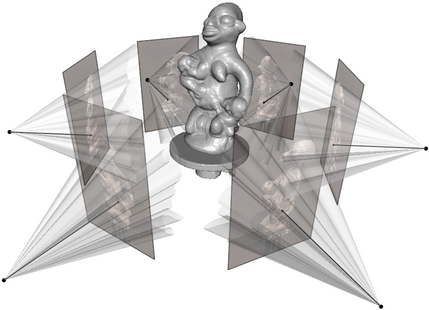
\includegraphics[width=0.2\textwidth]{relatedwork/mvs.png}} &
\raisebox{-0.75\height}{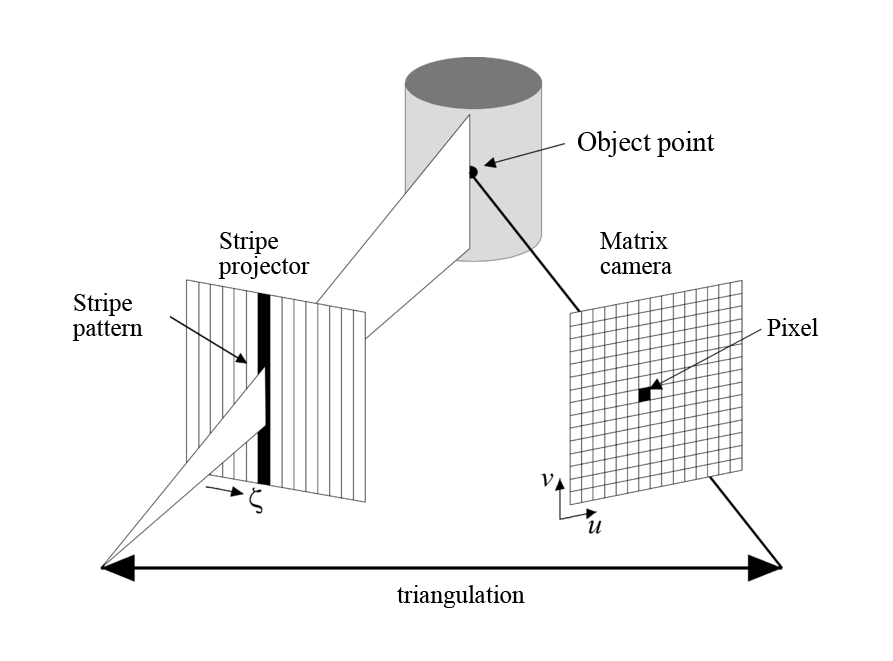
\includegraphics[width=0.2\textwidth]{relatedwork/sl.jpg}} &
Stereo correspondence &
Texture, Albedo, Specular \\
Shape from Intensity & 
\raisebox{-.75\height}{
\includegraphics[width=0.15\textwidth]{relatedwork/sfs.png}} &
\raisebox{-.75\height}{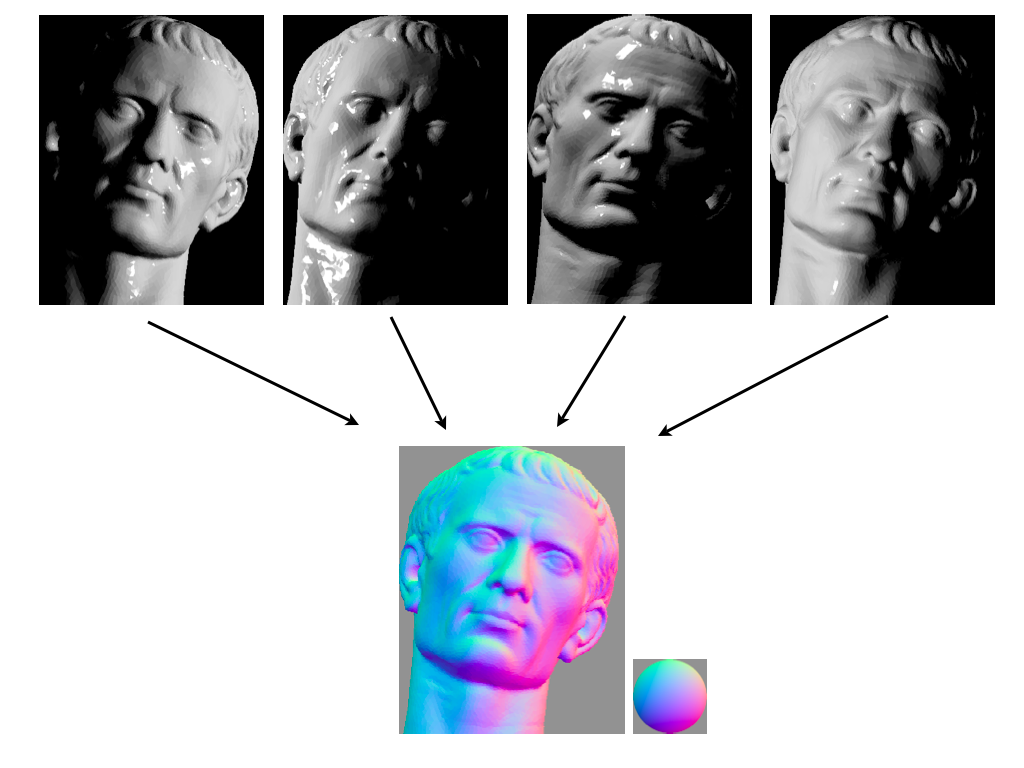
\includegraphics[width=0.2\textwidth]{relatedwork/ps.png}} &
Shading variation &
Albedo, Specular, Geometry \\
Shape from Silhouette &
\raisebox{-.75\height}{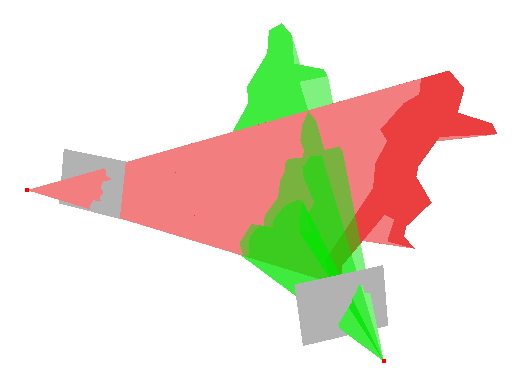
\includegraphics[width=0.2\textwidth]{relatedwork/vh.jpg}} &
\raisebox{-.75\height}{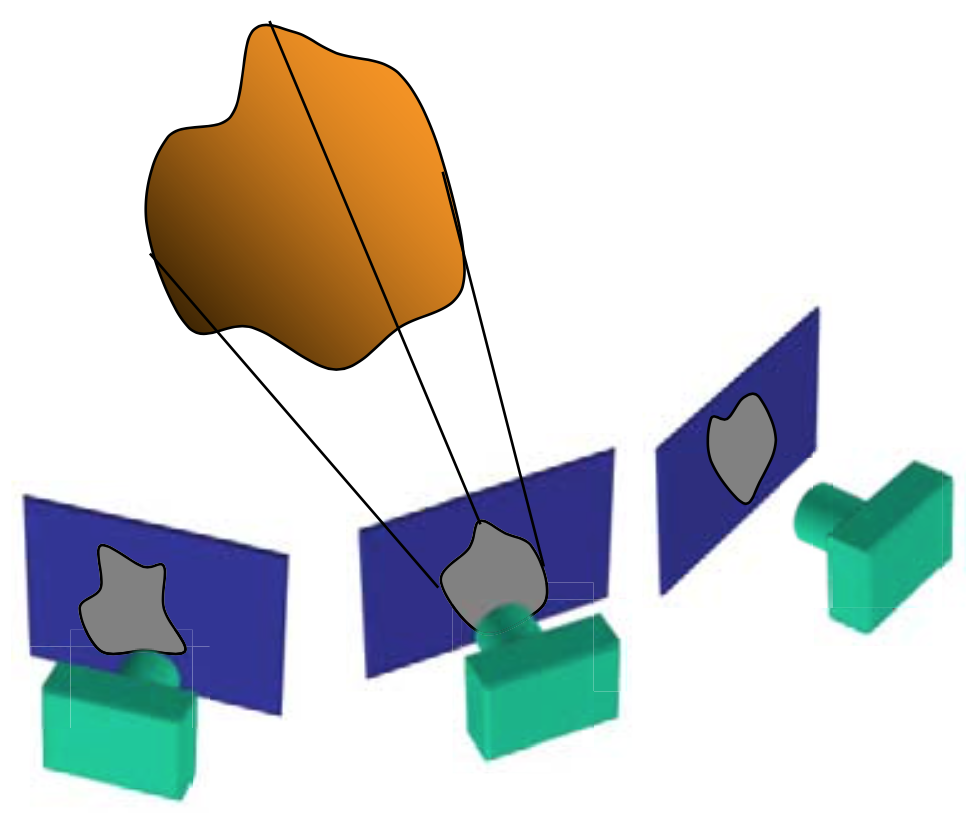
\includegraphics[width=0.2\textwidth]{relatedwork/vh_1.png}} &
Silhouette &
Geometry\\
\end{tabular}
\caption{Three classes of algorithms with examples, visual cues used for reconstruction, and potential problems.}
\label{fig:algo_class}
\end{figure}

\subsection{Stereo}
Stereo correspondence is one of the most widely used visual cues in 3D vision. Passive methods, including stereoscopy, trinocular stereo, and MVS, identify correspondences across different views, and estimate the 3D point by triangulation. However these passive approaches suffer from uniform or periodic surfaces. Active techniques attempt to overcome the correspondence problem by replacing one of the cameras with a controllable illumination source, e.g., single-point laser, slit laser scanner, temporal or spatially modulated Structured Light (SL), etc. Here we refer readers to the survey article by \citeauthor{blais2004review} for recent developments of active methods. We classify one of the most widely used passive methods, MVS algorithms, based on the taxonomy proposed in~\cite{seitz2006comparison}, which divides the field into four classes based on reconstruction method, and categorize one of the active methods, Structured Light technique, by projection patterns.

\subsubsection{Passive method: Multi-View Stereo}
\textbf{Volumetric stereo} algorithms compute a cost function in a 3D volume, then extract a surface from this volume. One successful example is voxel colouring, which traverses a sampled 3D space in ``depth-order'' to identify voxels that have a unique colouring, constant across all possible interpretations of the scene~\cite{seitz1997photorealistic}. Another thread of work formulates the problem in the Markov Random Field (MRF) framework and extracts the optimal surface by Graph-Cut algorithms~\cite{roy1998maximum,vogiatzis2005multi,vogiatzis2007multiview}.

\textbf{Surface Evolution} algorithms work by iteratively evolving a volume or surface to minimize a cost function. This includes methods based on voxels, level set, and surface meshes. The Space Carving technique achieves a least-commitment shape~\cite{marr1982vision} by iteratively removing inconsistent voxels from the scene~\cite{kutulakos2000theory}. Level-set techniques cast the problem as a variational problem, and use a set of PDE's as cost functions, which are deformed from an initial set of surfaces towards the detected objects~\cite{faugeras2002variational}. Other approaches use a deformable model and represent the scene as surface meshes that moves as a function of internal and external forces~\cite{esteban2004silhouette}. \citeauthor{hiep2009towards} presented a visibility-based method that transforms a dense point cloud into a surface mesh, which is fed into a mesh-based variational refinement that captures small details, smartly handling photo-consistency, regularization and adaptive resolution.

% Level-set based techniques minimize a set of partial differential equations defined in a volume. Like space carving methods, level-set methods typically start from a initial volume and shrink inward, or outward if the cost function is minimized. \citeauthor{faugeras2002variational} proposed a novel geometric approach based on variational principle, from which a set of PDE's can be deduced. The level set method is used to deform an initial set of surfaces towards the objects to be detected. However, level-set is no long a popular MVS technique, because high quailty models with correct topology can be directly computed from photo-consistency functions without the refinement steps.

\textbf{Region Growing} algorithms start with a sparse set of scene points, then propagate these points to spatial neighbours, and refine the cost function with respect to position and orientation of the points. \citeauthor{otto1989region} proposed one of the first work on region growing stereo search~\cite{otto1989region}. The idea of this algorithm is as follows: start with an approximate match between a point in one image and a point in another, use an adaptive least-squares correlation algorithm to produce a more accurate match, and use this to predict approximate matches for points in the neighbourhood of the first match. \citeauthor{lhuillier2002match} proposed a two-view quasi-dense approach, which first sorts a list of point correspondences into a list of seed points by correlation score. Next, at each step of the propagation, a `best' seed point is chosen. Lastly, in the immediate spatial neighbourhood of this seed point, new potential matches are checked and the best points are added to the current list of seed points~\cite{lhuillier2002match,lhuillier2005quasi}. This ``best-first'' strategy guarantees convergence by choosing only new matches that have not yet been selected. Further, a patch based approach is proposed that undergoes multiple iterations of matching, propagation, and filtering~\cite{furukawa2010accurate}. A stereoscopic approach called PatchMatch Stereo, which is inspired by an approximate nearest neighbour matching algorithm called PatchMatch~\cite{Barnes:2009:PAR}, starts by randomly assigning an oriented plane to each pixel in two views. Next, each pixel is taken through three iterations of propagation and refinement. The plane is propagated to spatial neighbours, the corresponding pixel from another view, and across time. It can achieve sub-pixel accuracy, but is computationally heavy and challenging for parallelism. There has been some efforts to apply PatchMatch Stereo to multi-view scenarios~\cite{galliani2015massively,uh2014efficient,zheng2014patchmatch}, and develop new propagation schemes to increase the computational efficiency~\cite{galliani2015massively}.
%[has nice math derivations] Shen, Accurate Multiple View 3D Reconstruction Using Patch-Based Stereo for Large-Scale Scenes\\

\textbf{Depthmap Merging} algorithms work by computing a per-view depthmap. By treating a depthmap as a 2D array of 3D points, multiple depthmaps can be considered as a merged 3D point cloud. A `winner-takes-all' approach uses a set of sampled depth values and picks the value with the highest photo-consistency score for each pixel independently. Uniform depth sampling may suffice for simple and compact objects. However, for complex and large scenes, a proper sampling scheme is crucial to achieve high speed and quality. More sophisticated cost functions are derived to account for occlusion or non-Lambertian effects which may add noise to the photo-consistency score~\cite{goesele2006multi,vogiatzis2007multiview}. In the case of severe occlusion, spatial consistency can be enforced under the assumption that neighbouring pixels have similar depth values. This can be formulated under the Markov Random Field (MRF) framework, where the problem becomes minimizing the sum of a unary $\Phi(\cdot)$ and pairwise term $\Psi(\cdot, \cdot)$. The unary term reflects the photo-consistency score of assigning a depth value $d_p$ from a set of depth value to the pixel $p$, whereas the pairwise term enforces the spatial regularization, and assigns the cost of setting depth label $k_p$, $k_q$ to a pair of neighbouring pixels $p$ and $q$, respectively.
$$
E(\{k_p\})= \sum_p \Phi(k_p) + \sum_{(p,q)\in\mathcal{N}}\Psi(k_p, k_q)
$$

MVS algorithms generally have a less strict requirement on the setup, and work relatively reliably in unconstrained environments. However, it suffers under the following two conditions:

\textbf{Lack of texture}: Multi-View Stereo algorithms take advantage of textural information to establish point correspondences across different views. Thus homogeneous surfaces pose great challenges to MVS algorithms. We have witnessed surprisingly good results on a textureless object ``Dino'' in the Middlebury MVS benchmark~\cite{seitz2006comparison}. It turns out that MVS algorithms are able to exploit very weak and intricate image textures, most of which come from shading or shadowing effects. However, these texture are so weak that images have to have very high quality.

\textbf{Non-Lambertian surface}: MVS algorithms require to observe the same surface patch from different angles in order to establish correspondences across views. Thus, the same surface patch needs to have similar or same appearance from different perspectives, and hence, most of the algorithms assume Lambertian reflectance. Pure Lambertian surfaces are rare in reality, but it is empirically verified that most MVS algorithms perform reasonably well on non-Lambertian surfaces. As long as the cameras can capture the diffuse reflectance component, then the photo-consistency function is able to identify and ignore images whose non-diffuse effects (e.g., specular highlights) are strong, then utilize the diffuse component in the remaining images. Further, there are some attempts to overcome this limitation, a pure passive methods was proposed that directly model and analyze non-Lambertian effects for MVS algorithms~\cite{jin2003multi,jin2005multi}.

\subsubsection{Active method: Structured Light}
To overcome the problem of lack of texture, one of the cameras in stereoscopy can be replaced by an illumination source, \eg a projector, which is called Structured Light technique. It is based on projecting a temporally or spatially modulated pattern onto a surface and viewing the illuminated surface from one or more points of view. The correspondence is easily detected from the projected and imaged pattern, which is triangulated to obtain the a 3D point. Each pixel in the pattern is assigned a unique codeword, and the codeword is encoded by using grey level, colour or geometric representations. Structured Light is classified based on the following coding strategy: temporal, spatial and direct codification~\cite{salvi2004pattern}. Temporal techniques generate the codeword by projecting a sequence of patterns. Spatial codification represents each codeword in a unique spatial pattern. Direct codification techniques define a codeword for every pixel, which is equal to its grey level or colour.

\textbf{Temporally encoded} SL projects a sequence of patterns successively onto the surface. The codeword for a given pixel is formed by a sequence of illumination values for that pixel across the projected patterns. This kind of pattern can achieve high accuracy due to two factors: 1) the codeword basis is small (e.g., two for binary pattern), therefore, each bit is easily distinguishable; 2) a coarse-to-fine strategy is used, and the position of the pixel becomes more precise as the patterns are successively projected. This technique can be further classified by the way pattern is encoded temporally: 1) binary codeword; 2) $n$-ary codeword; 3) Gray-code combined with phase shifting; 4) hybrid techniques. More details are available in this review~\cite{salvi2004pattern}.

\textbf{Spatially encoded} techniques concentrate all coding into a unique pattern. The codeword that labels a certain pixel is obtained from the neighbourhood of pixels around it. Normally, the visual features gathered in a neighbourhood are the intensity or colour of the pixels or groups of pixels around it.

\textbf{Directly encoded} methods represent the codeword in each pixel directly. To achieve this, we need to use either a large range of colour values or introduce periodicity. However, this kind of pattern is highly sensitive to noise because the ``distance'' between codewords is nearly zero. Moreover, the perceived colour depends not only on the projected colour, but also the intrinsic colour of the surface. Therefore, reference images must be taken to eliminate the effect of surface colour. This kind of coding can be further classified as: 1). codification based on grey levels; 2). codification based on colour. More details are available in review~\cite{salvi2004pattern}.

Structured Light techniques overcomes the lack of texture problem by actively projecting a pattern onto the surface. However, it still suffers under the following conditions:

\textbf{Low surface albedo} poses a great challenge to active methods, such as SL, which utilize reflected light to establish correspondences across different views. Regardless of which projection pattern is used, the most critical component of any SL system is the decoding process, which retrieves per-pixel codeword from the imaged projection pattern. Thus, the surface albedo needs to be strong enough so that sufficient amount of reflected light can reach the camera sensor.

\textbf{Non-Lambertian surfaces} exhibit strong reflection in the specular direction. Images of such surfaces are challenging to interpret due to the bright points or highlights, which makes the projected pattern indistinguishable in these areas. Thus, it is impossible to decode the pixels exhibiting specular effects.

\textbf{Concavity} is the cause of global light transport, such as inter-reflection, which results in surface patches receiving light from sources other than the projector. Thus, the intensity value or colour of a pixel becomes noisier, which seriously affects the accuracy of decoding process.

\subsection{Shading}
Shading variation is an effective visual cue for retrieving shape of a surface. Shading variation depends on surface geometry (surface orientation), reflectance (material), and lighting (illumination). This is generally an ill-posed problem because different shapes illuminated under different light conditions may produce the same image. It becomes possible to estimate surface orientation once the reflectance property and illumination are known. This technique of estimating surface shape by shading variation is called Shape from Shading. However, this technique requires strict constraints on surface geometry since only one input image is used, which leads to a novel technique called Photometric Stereo in which surface orientation is determined from two or more images. The idea of Photometric Stereo is to vary the direction of the incident illumination between successive views while holding the viewing direction constant. This provides enough information to determine surface orientation at each pixel~\cite{woodham1979photometric}. This technique can produce a surface normal map with the same resolution of the input image, \ie to produce the pixel-wise surface normal map. Since the coefficients of the normal map are continuous, the integrated height map can reach an accuracy that cannot be achieved by any triangulation methods. Therefore, the Photometric Stereo technique is more desirable if the intrinsic geometric details are of great importance.

\subsubsection{Shape from Shading}
The problem of recovering the shape of a surface from intensity variation is first proposed by Horn~\cite{horn1970shape}. It assumes that the surface under consideration is of a uniform albedo and reflectance, and that the direction of the single distant light source is either known or can be calibrated by the use of a reference object. Thus the intensity $I(x,y)$ becomes purely a function of the local surface orientation. The information of reflectance, illumination, and viewing geometry can be combined into a single function called reflectance map $R(p, q)$, that relates surface orientation directly to image intensities:
\begin{align*}
I(x, y) &= R(p(x, y), q(x, y))
% I(x, y) &= \rho(\vec{n},\vec{l})\vec{n}^\top\vec{l} \quad (\text{Lambertian model})
\end{align*}
where $(p, q) = (z_x, z_y)$ are surface gradients. Unfortunately, there are more unknown (per-pixel gradient) than there are measurements (per-pixel intensity). More specifically, surface orientation has two unknowns($p, q$) whereas measurements of the brightness at a single pixel only provide one constraint. Thus, additional information regarding the surface reflectance and illumination, as well as constraints on surface geometry, such as smoothness or integrability are required to estimate $(p, q)$. One common used constraint is smoothness:
\begin{align*}
\int p_x^2 + p_y^2 + q_x^2 + q_y^2 \mathrm{d}x\mathrm{d}y = \int \|\nabla p\|^2+\|\nabla q\|^2 \mathrm{d}x\mathrm{d}y
\end{align*}
Another is the integrability constraint:
\begin{align*}
\int(p_y-q_x)^2 \mathrm{d}x\mathrm{d}y
\end{align*}
since for a valid depth $z(x, y)$ with $(p, q)=(z_x, z_y)$, we have $p_y=z_{xy}=z_{yx}=q_x$.

% The Shape from Shading problem is an ill-posed problem since it need to solves for two unknown (surface normal, gradient) with only one input (per-pixel intensity). With additional constraints regarding the surface smoothness, this problem can potentially be solvable.

Most shape from shading algorithms assume that the surface under consideration is of a uniform albedo and reflectance, and that the light source directions are either known or can be calibrated by the use of a reference object. Thus, they are applicable to textureless surfaces with uniform and known albedo. Besides, a tedious calibration step needs to be carried out to estimate light direction and intensity. However, even by assuming the simplest reflectance model, Lambertian reflectance, the survey by Zhang~\cite{zhang1999shape} demonstrated that SfS algorithms generally perform poorly, and none performs well in all cases.

% \textbf{Texture: textureless}
% Typical SfS algorithms assume surfaces with uniform and known albedo, \ie textureless surfaces.

% \textbf{Brightness}
% Active methods such as SfS utilize reflected light to estimate surface depth or orientation information. In this case, the intensity variation is used to estimate surface normal, thus the surface should have sufficiently high albedo, otherwise, the intensity variation would be hard to detect.

% \textbf{Reflectance}
% Though other reflectance models are feasible, typical SfS algorithms assume Lambertian reflectance model. The reason is that surface lightness is directly related to surface orientation and reflectance model once the light source and viewing direction are fixed. This is generally an ill-posed problem even with Lambertian model since there is only one intensity value per pixel to solve for surface orientation, which has two DoF. 

% \textbf{Concavity}
% Typical SfS algorithms can not deal with effects caused by global light transport, such as cast shadow, inter-reflection, and so on. The surface lightness would be corrupted by light transported from other surface facets. Thus, objects exhibit any form of concavity will pose great challenge to SfS algorithms.

\subsubsection{Photometric Stereo}
The \textbf{Classical Photometric Stereo}, first proposed by Woodham~\cite{woodham1980photometric}, utilized multiple light sources from different directions to overcome the ambiguity of Shape from Shading. Assuming Lambertian reflectance, $P$ pixels per image, and $Q$ illumination directions, the intensity of the $i$th pixel under $j$th illumination is
\begin{align*}
I_{i,j} &= \rho_i\vec{n}_i^\top \vec{l}_j\\
\Rightarrow\mathbf{I} &= \mathbf{N}^\top \mathbf{L}
\end{align*}
where $\mathbf{I}\in \mathbb{R}^{P\times Q}$ stores the pixel intensity from all images. Each column contains pixels from each image while each rows contains intensity of each pixel under all illumination conditions. $\mathbf{N}\in \mathbb{R}^{P\times3}$ encodes the albedo-scaled surface normal for each pixel, \ie $N_{i, :} = \rho_i\vec{n}_i^\top$. $\mathbf{L} \in \mathbb{R}^{3\times Q}$ encodes the light source directions, \ie $L_{:, j} = \vec{l_j}$. This surface reflectance, \ie spatially varying albedo $\rho_i$, and the normal $n_i$ can be estimated by
\begin{align*}
\mathbf{N} &= \mathbf{I}\mathbf{L}^{+}\\
\Rightarrow\rho_i &= \|\mathbf{N}_{i,:}\|\\
\Rightarrow n_i &= \frac{\mathbf{N}_{i,:}^\top}{\|\mathbf{N}_{i,:}\|}
\end{align*}

Thus, the problem of estimating shape of a Lambertian surface under known lighting conditions has a simple solution. However, this algorithm fails to work once these constraints are violated. Thus, past research efforts have been focused on generalizing various assumptions made by classical photometric stereo. For the camera assumption, orthographic projection can be achieved by using a lens with long focus and placing the objects far from the camera. The nonlinear response can be solved by performing radiometric calibration. The shadow and other global light transportation are a few of the sources of errors, where some approaches consider them as outliers and remove them before normal estimation. The reflectance and lighting assumptions, however, are the most complicated since the reflectance properties depends on material property and microscopic structure. Further, lighting can have either an arbitrary or fixed position, orientation, and intensity. Therefore, research on Photometric Stereo are generally on two directions: 1) generalization of reflectance; 2) generalization of lighting conditions. A summary of assumptions made by various classes of PS algorithms are presented in Table~\ref{tab:ps_assumptions}.
\begin{table}[!htbp]
  \centering
  \begin{tabular}{p{2cm}|cp{4cm}c}
  \toprule
  \textbf{Category} & Camera & Light source & Reflectance \\
  \midrule
  Classical PS & Orthographic & Directional, known intensity and direction & Lambertian \\
  Generalized lighting PS & Orthographic & Unknown intensity and direction, ambient & Lambertian \\
  Generalized reflectance PS & Orthographic & Distant, known intensity and direction & Non-Lambertian \\
  \bottomrule
  \end{tabular}
  \caption{Assumptions made by different classes of photometric stereo.}
  \label{tab:ps_assumptions}
\end{table}

\textbf{Generalization of Lighting} 
It is possible to estimate the surface orientation without knowing light directions, a case also known as \textit{uncalibrated Photometric Stereo}, see Table~\ref{tab:ps_assumptions}. Most uncalibrated techniques assume Lambertian techniques and are based on factorization technique proposed in \cite{hayakawa1994photometric}. Recall the irradiance equation:
$$
\mathbf{I}=\mathbf{N}^\top \mathbf{L}
$$
However, an infinite number of candidates $\hat{N}$ and $\hat{L}$ make the above equality met. In fact, any invertible $3\times 3$ matrix $G$ defines a candidate pair $\hat{N} = N\cdot G, \hat{L}=G^{-1}L$. Thus the normal $N$ and light source direction $L$ can only be recovered up to a linear transformation. It has been shown that only a 3-parameter subset of these transformations, known as the Generalized Bas-Relief (GBR) ambiguity, preserve surface integrability~\cite{belhumeur1999bas}.

Other generalized lighting conditions are any situations other than the ideal case of using a single distant point light source in a dark room, such as natural ambient light, multiple point light sources with or without ambient lighting, etc. To make the problem more tractable, the reflectance model should no longer be a general one, as this involves too many degrees of freedom that results in many different shapes with incorrectly estimated general reflectance and incorrectly estimated general lighting.

\textbf{Generalization of Reflectance} This direction of research has been to relax the assumption of Lambertian reflectance. This can be broadly divided into four classes of algorithms.

\textit{Outlier rejection} approach assumes that Non-Lambertian reflectance can be well approximated by the sum of diffuse and specular lobe. The specular pixels are considered as outliers in ~\cite{coleman1982obtaining} and \cite{barsky20034}. Others assume that the colour of the specular lobe differs from that of the diffuse lobe, which allows the separation of the specular and diffuse components~\cite{mallick2005beyond,sato1994temporal,schluns1993photometric}.

\textit{Reference object} approach uses a reference object that has similar material as the target object. This is proposed in~\cite{silver1980determining} and later revisited in~\cite{hertzmann2005example}. The idea is that surface points with same orientation give similar intensity values under similar reflectance and lighting. It can deal with arbitrary BRDFs as long as the reference and target object has the same material. It can handle spatially-varying BRDFs as long as there are multiple reference objects. Each reference object serves as a ``basis'' BRDF, and the BRDF at any point on the target object can be approximated as a linear combination of the basis BRDFs.

\textit{Parametric reflectance model} approach builds upon the idea that an arbitrary BRDF can be approximated by ``basis'' BRDFs, and replaces the reference objects with sophisticated BRDF models. An isotropic Ward model is used as basis BRDF, and the surface orientation and parameters of the reflectance models are estimated iteratively~\cite{goldman2010shape}.

\textit{Invariants of BRDF} approach exploits various physical properties of BRDFs. While parametric reflectance models are very good at reducing the complexity of BRDFs, they are usually only valid for a limited class of materials. An alternative is to exploit the invariants of BRDFs, typically including energy conservation, non-negativity, Helmholtz reciprocity, isotropy, and so on~\cite{zickler2002helmholtz,alldrin2007toward}.

Photometric Stereo can work extremly well under certain constrained conditions. However, it generally performs poorly once the aforementioned assumptions are violated: the classical PS and generalized reflectance PS fail to work under uncalibrated light conditions. The generalized lighting PS only handle Lambertian surfaces under uncalibrated lighting conditions, but only achieves estimation up to a linear transformation; the classical PS and generalized lighting PS fail to work under generalized reflectance conditions; and lastly, most PS algorithms fail to work on conditions of generalized lighting and reflectance, one approach that has been proved to work is to place multiple reference objects in the scene with the target object as proposed by~\cite{hertzmann2005example}.

% \subsubsection{Limits: PS}
% \textbf{Texture} 
% Though SfS algorithms require uniform and known albedo, typical PS algorithms can be used easily on surfaces with spatially varying albedo. For instance, the albedo-scaled normal can be estimated, then the albedo is retrieved as the magnitude of the scaled normal~\cite{woodham1980photometric}.

% \textbf{Brightness} 
% Active methods such as PS utilize reflected light to estimate surface depth or orientation information. In this case, PS algorithms work more reliably on surfaces with sufficiently strong albedo. This is because the algorithm exploits the intensity variation as a visual cue, which is more challenging to detect on surfaces with low intensity values.

% \textbf{Reflectance} % Lambertian PS: uniform reflectance
% The Lambertian PS algorithms can be divided into two groups: calibrated, and uncalibrated method. The classical PS proposed by Woodham~\cite{woodham1980photometric} can be considered as calibrated Lambertian PS. Later, more uncalibrated Lambertian PS algorithms have been proposed to avoid this tedious process.

% \textbf{Convexity} 
% Active methods that assumes a \textbf{local interaction model}, such as most PS algorithms, can work more reliably on surfaces without casting shadow and inter-reflection. Thus surfaces with concavities pose a great challenge for this type of techniques since the indensity can be affected by other surface patches.

% [Some other papers to read] \\
% - R. J. Woodham. Photometric method for determining sur-
% face orientation from multiple images.\\
% 1. joint recovery of unknown shape and reflectance\\
% - N. Alldrin, T. Zickler, and D. Kriegman. Photometric stereo with non-parametric and spatially-varying reflectance.\\
% - D. Goldman, B. Curless, A. Hertzmann, and S. Seitz. Shape and spatially-varying BRDFs from photometric stereo.\\
% - T. Higo, Y. Matsushita, and K. Ikeuchi. Consensus photometric stereo.\\
% - B.Shi,P.Tan,Y.Matsushita,and K.Ikeuchi. Elevationangle from reflectance monotonicity: Photometric stereo for general isotropic reflectances.\\
% - BOXIN SHI's PhD thesis\\
% - Satoshi Ikehata's PhD thesis\\
% 2. a less restrained capture setup with arbitrary and unknown illumination\\
% - H. Hayakawa. Photometric stereo under a light source with arbitrary motion\\
% - T. Papadhimitri and P. Favaro. A new perspective on uncalibrated photometric stereo\\
% - B. Shi, Y. Matsushita, Y. Wei, C. Xu, and P. Tan. Self-calibrating photometric stereo\\
% 3. combine both directions\\
% - A.Hertzmannand S.Seitz.Shapeandmaterialsbyexample: a photometric stereo approach.\\
% - A. Hertzmann and S. Seitz. Example-based photometric stereo: shape reconstruction with general, varying BRDFs.\\
% - W. M. Silver. Determining shape and reflectance using mul- tiple images. Master’s thesis, MIT, 1980.\\

\subsection{Silhouette}
In some cases, it's an easy task to perform a foreground segmentation of the object of interest, which leads to a class of techniques that reconstructs a 3D volumetric model from the intersection of the binary silhouettes projected into 3D. The resulting model is called a \textit{visual hull}.

The basic idea of shape from silhouette algorithms is that the object lies inside the intersection of all visual cones back-projected from silhouettes. Suppose there are multiple views $V$ of the target object. From each viewpoint $v\in V$, the silhouette $s_v$ can be extracted, which is the region including the object's interior pixels and delimited by the line(s) separating the object from the background. The silhouette $s_v$ are generally non-convex and can represent holes due to the geometry of the object. A cone-like volume $cone_v$ called (truncated) extended silhouette is generated by all the rays starting at the centre of projection and passing through all the points of the silhouette. The target object is definitely internal to $cone_v$ and this is true fro every view $v'\in V$; it follows that the object is contained inside the volume $c_V=\cap_{v\in V}c_v$. As the size of the $V$ goes to infinity, and all possible views are included, $c_V$ converges to a shape known as the \textit{visual hull} $vh$ of the target object.

% Some approaches first approximate each silhouette with a polygonal representation and then intersect the resulting faceted conical regions in 3D space to produce polyhedral models, which can be later refined using triangular splines. Other approaches use voxel-based representations, usually encoded as octrees, because of the resulting time-space efficiency.

% [computational complexity] intersection of many volumes can be slow. Simple polyhedron-polyhedron intersection algorithms are inefficient. To improve performance, most methods 1) quantify volumes, 2) perform intersection computation in 2D instead of 3D.

\textbf {Voxel based methods} 
First the object space is split up into a 3D grid of voxels; each voxel is intersected with each silhouette volume; only voxels that lie inside all silhouette volumes remain part of the final shape.

\textbf{Marching intersections based methods} 
The marching intersection (MI) structure consists of 3 orthogonal sets of rays, parallel to the $X$, $Y$, and $Z$ axis, which are arranged in 2D regular arrays, called the $X-rayset$, $Y-rayset$, $Z-rayset$ respectively. Each ray in each rayset is projected to the image plane to find the intersections with the silhouette. These intersections are un-projected to compute the 3D intersection between the ray and the extended silhouette on this ray. This process is repeated for each silhouette, and the un-projected intersections on the same ray are merged by the boolean AND operation.

Once the MI data structure representing the intersection of all extended silhouettes, a triangular mesh is extracted from it. This is done by the MI technique proposed in~\cite{rocchini2001marching} which traverses the ``virtual cells'' implicitly defined by the MI, builds a proper marching cube (MC) entry for them that in turn is used to index a MC's lookup table.

\textbf{Exact polyhedral methods} 
The silhouette is converted into a set of convex or non-convex 2D polygons with holes allowed. The resulting visual hull with respect to those polygonal silhouettes is a polyhedron. The faces of this polyhedron lie on the faces of the original cones. The faces of the original cones are defined by the centre of projections and the edges in the input silhouettes. The idea of this method is: for each input silhouette $s_i$ we compute the face of the cone. Then we intersect this face with cones of all other input silhouettes, \ie a polygon-polyhedron intersection. The result of these intersections is a set of polygons that define the surface of the visual hull.

% \subsection{Image based method}
% \begin{itemize}
% \item this algorithm will only produce renderings of a visual hull from any view
% \item every pixel in the desired output image is back-projected to form a 3D ray
% \item each of those rays is intersected with each of the input silhouettes in the same way as the rays in the marching intersections method
% \item a pixel in the output image is inside the new rendering of the visual hull if its ray has any segments left in it that are intersecting the visual hull. The depth of these pixels is known from the depth of the nearest entry point on the ray.
% \end{itemize}

Visual Hull algorithms don't rely on material properties as long as the foreground of the image can be reliably segmented, thus is applicable for objects with arbitrary reflectance properties. However, it fails to carve the concavities on the object surface, thus is unsuitable for concave objects.

% All of the cues above are most widely used ones, and achieved decent results. These following two cues haven't resulted in as much success. Therefore, we only discuss the general idea rather than the technical details.

% \subsection{Texture}
% The basic principle behind shape from texture is the \textit{distortion} of the individual texel. In general, the image formation process introduces three distortion effects: the \textit{distance effect}, which makes objects in view appear larger when they are closer to the image plane; the \textit{position effect} which makes objects appear differently when the angle between the line of sight and the image plane different; and the \textit{forshortening effect}, which distort the objects depending on the angle between the surface normal and the line of sight. Besides, different effects take place under different projection models: the orthographic projection captures only the foreshortending effect whereas the perspective projection captures all three. Therefore, shape from texture methods which use orthographic projection are valid only in a limited domain, where the other two effects can be ignored, and the perspective model captures all three effects, but the resulting algorithms are complicated and involves the solution of nonlinear equations.
% \begin{figure}[h]
% \centering
% 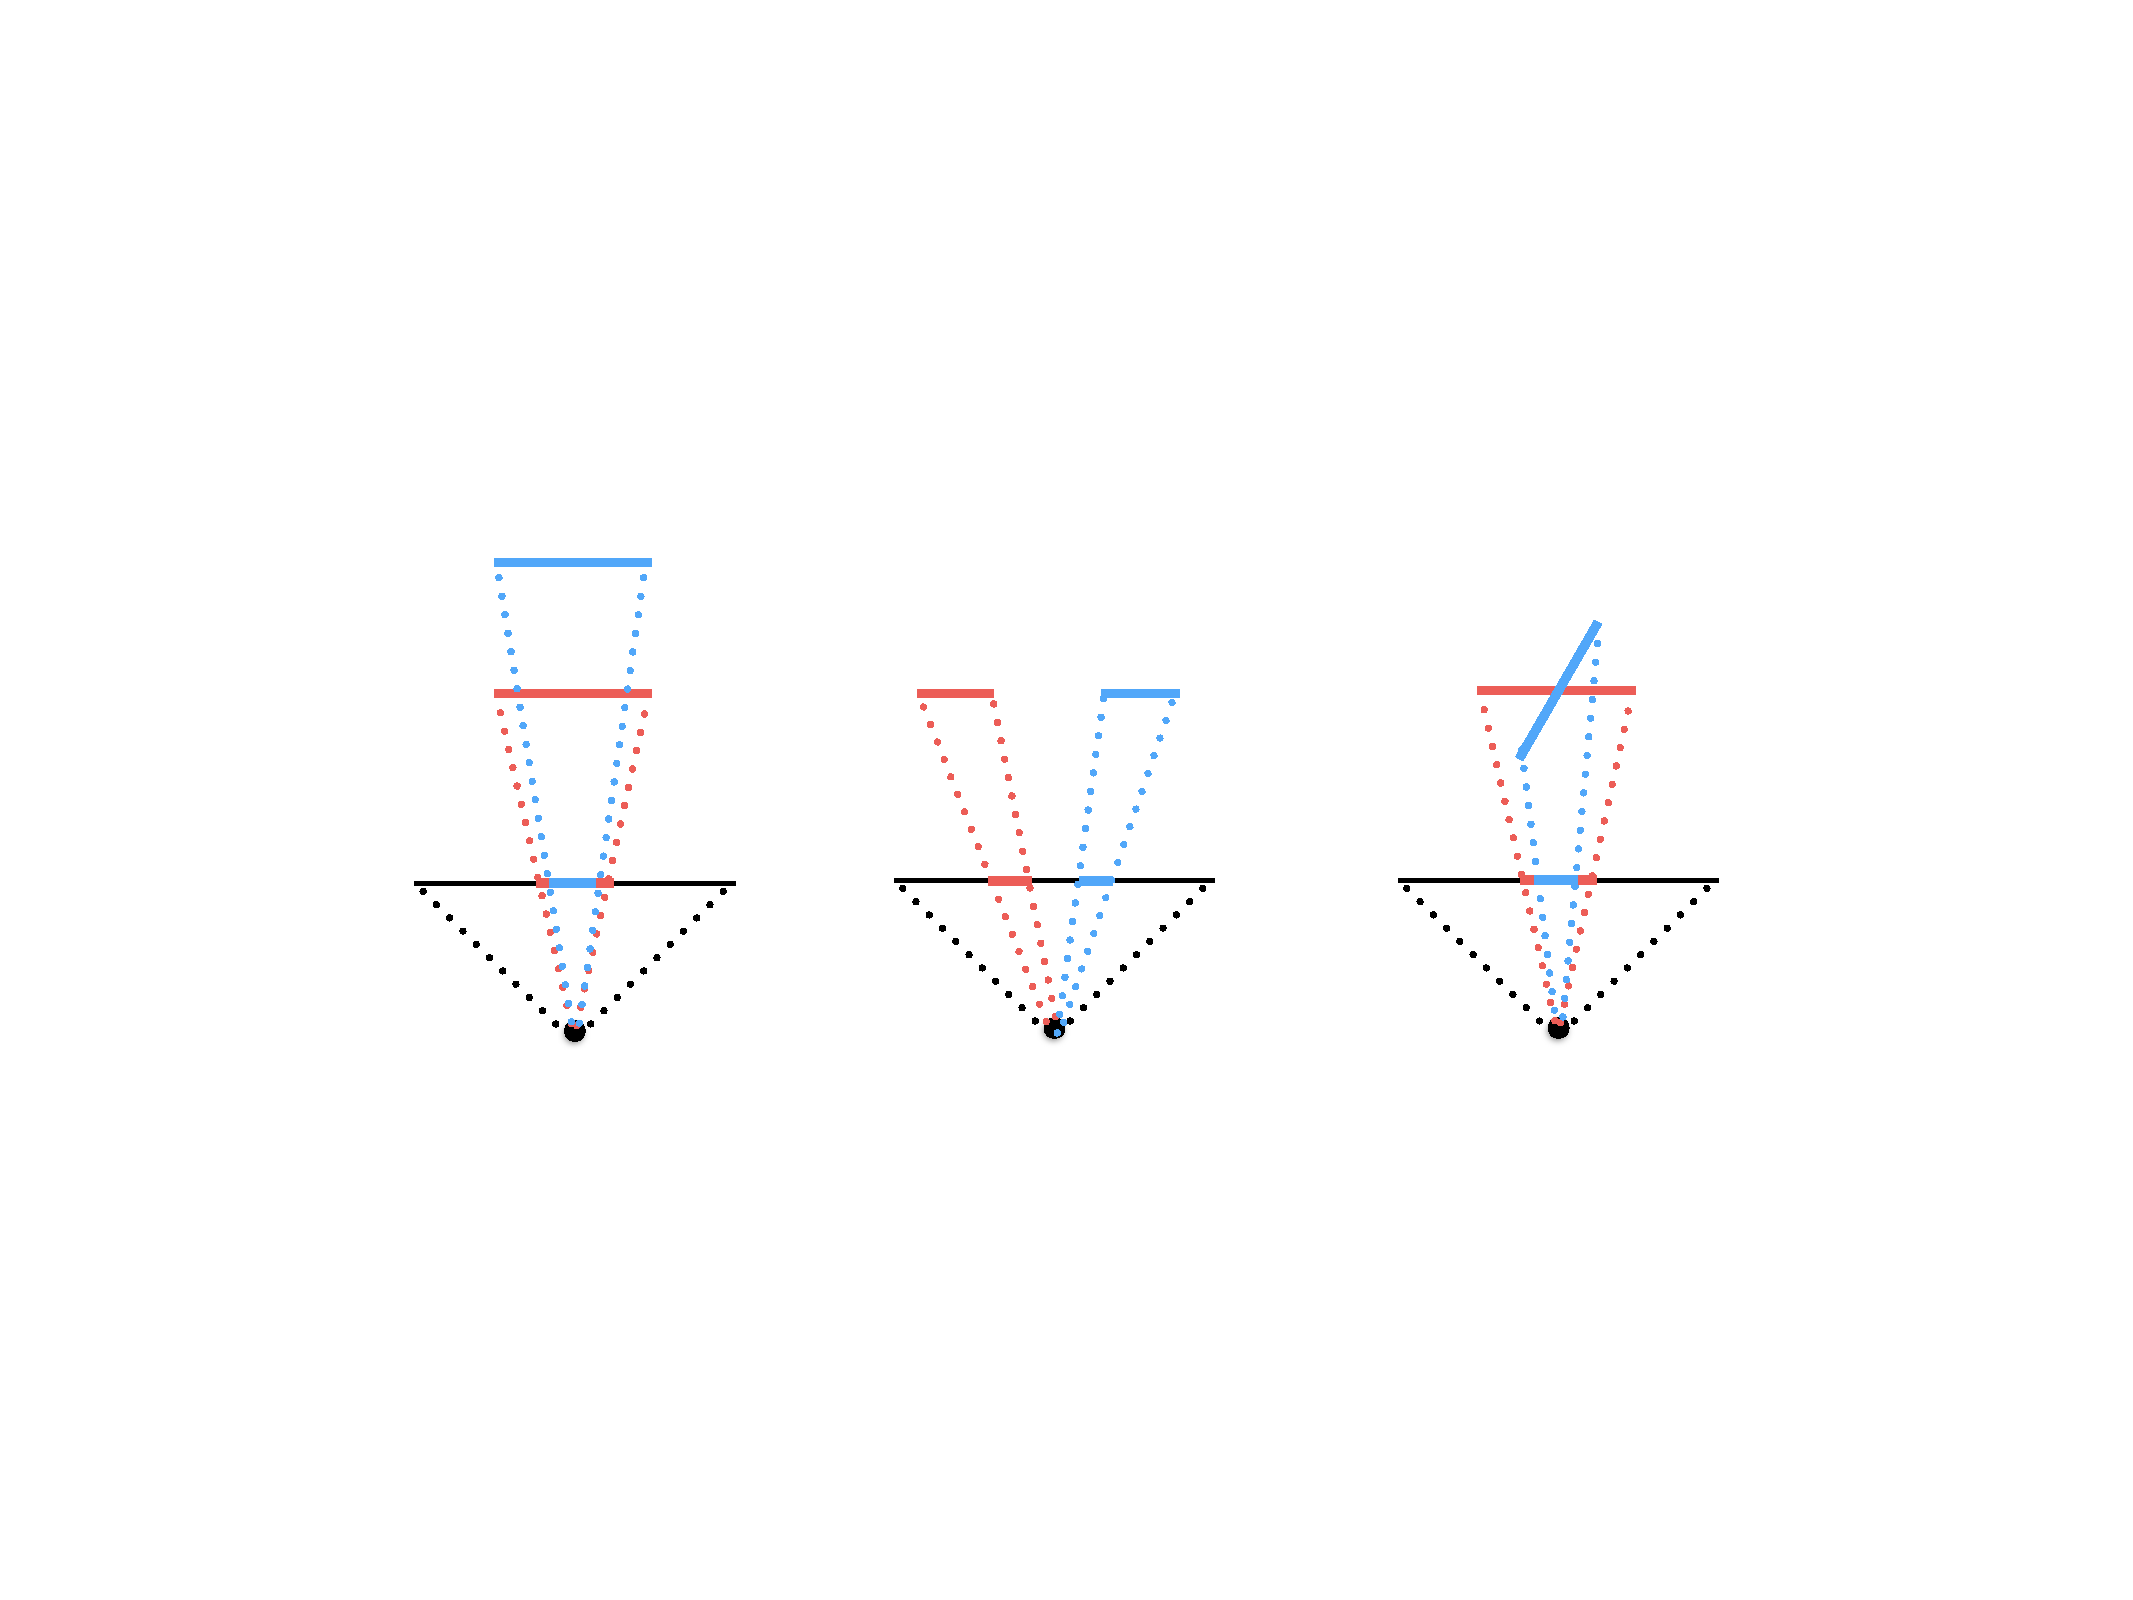
\includegraphics[width=0.8\textwidth]{relatedwork/tex_dist}
% \caption{Three distortion effect: distance distortion, position distortion, and foreshortening distortion.}
% \label{fig:tex_dist}
% \end{figure}

% To calculate the surface curvature at any point is far from trivial. Therefore, the surface shape is reconstructed by calculating the surface orientation (surface normal). A map of surface normals specifies the surface's orientation only at the points where the normals are computed. But, assuming that the normals are dense enough and the surface is smooth, the map can be used to reconstruct the surface shape.

% \subsection{Defocus}
% \textbf{Shape from focus}
% A strong cue for object depth is the amount of blur, which increases as the object moves away from the camera's focusing distance. As shown in Figure~\ref{fig:thin_lens}, moving the object surface away from the focus plane increases the circle of confusion.

% \begin{figure}[h]
% \centering
% 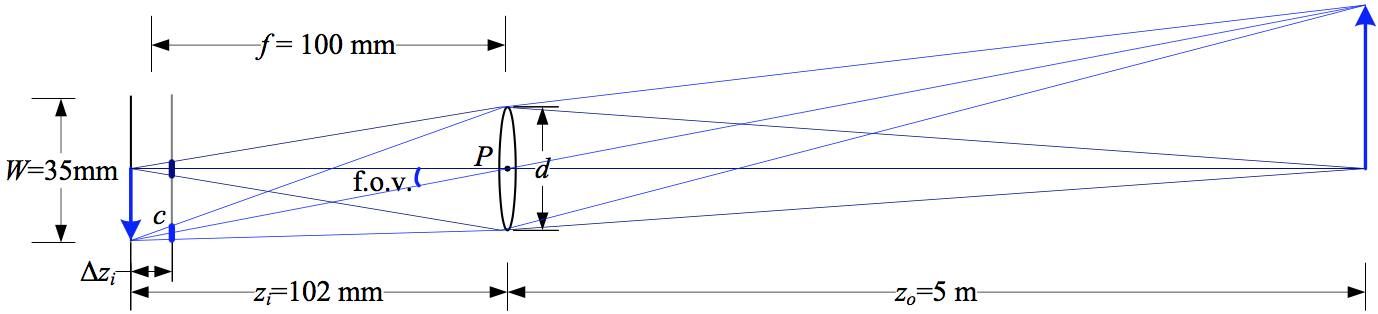
\includegraphics[width=0.8\textwidth]{relatedwork/thin_lens}
% \caption{A thin lens of focal length $f$ focuses the light from a plane a distance $z_0$ in front of the lens at a distance $z_i$ behind the lens, where $\frac{1}{z_o}+\frac{1}{z_i}=\frac{1}{f}$. If the sensor plane moved forward $\Delta z_i$, the image are no longer in focus and the \textit{circle of confusion} $c$ depends on the distance of the sensor plane motion $\Delta z_i$ relative to the lens aperture diameter $d$.}
% \label{fig:thin_lens}
% \end{figure}

% Figure~\ref{fig:thin_lens} shows the basic geometric image formation. The relationship between the object distance $z_o$, focal distance of the lens $f$, and the image distance $z_i$, is given by the Gaussian lens law:
% $$
% \frac{1}{z_o}+\frac{1}{z_i}=\frac{1}{f}
% $$
% All light rays that are radiated from the object and intercepted by the lens to converge at a single point on the image plane, thus a \textit{focused} image $I_f(x, y)$ is formed on the image plane. If, however, the sensor plane does not coincide with the image plane and is displaced from the image plane by a distance $\Delta z_i$, the energy received from the object is uniformly distributed over a circular patch on the sensor plane. The relationship between the radius $c$ of the circle of confusion and the sensor displacement $\Delta z_i$ is as follows:
% $$
% c = \frac{\Delta z_i r}{z_i}
% $$
% where $r$ is the radius of the lens. If we assume that the radius $c$ of the circle of confusion is independent of the position of the object point. Therefore, the \textit{defocused} image $I_d(x, y)$ formed on the sensor plane can also be obtained by convolving the focused image $I_f(x, y)$ with a circular symmetric ``pillbox'' filter
% $$
% I_d(x, y)=p(x, y)*I_f(x, y)
% $$
% where
% $$
% p(x, y) = \begin{cases}
%     \frac{1}{\pi r^2}       & \quad \text{if } x^2+y^2\leq r^2\\
%     0  & \quad \text{otherwise}\\
%   \end{cases}
% $$
% The defocused images can be obtained in three ways: by displacing the sensor with respect to the image plane, by moving the lens, or by moving the object with respect to the object plane. The first two ways cab cause the following problems:
% \begin{itemize}
% \item The magnification of the system varies, thereby causing the image coordinates of the object points to change.
% \item The area on the sensor plane over which light energy is distributed varies, thereby causing a variation in image brightness.
% \end{itemize}
% To address this issue, the degree of focus is changed by moving the object with respect to a fixed configuration of the optical system and sensor. This approach ensures that the focused areas of the image are always subjected to the same magnification.

% The idea is as follows: the stage is moved in increaments of $\Delta d$, and an image is captured at each stage position ($d=n\Delta d$). By studying the behaviour of the focus measure, an interpolation method is used to compute the accurate depth estimates from a small number of focus measures. An important feature of this method is the local nature, the depth estimate at an image point is computed only from focus measures recorded at that point.
% \begin{figure}[h]
% \centering
% 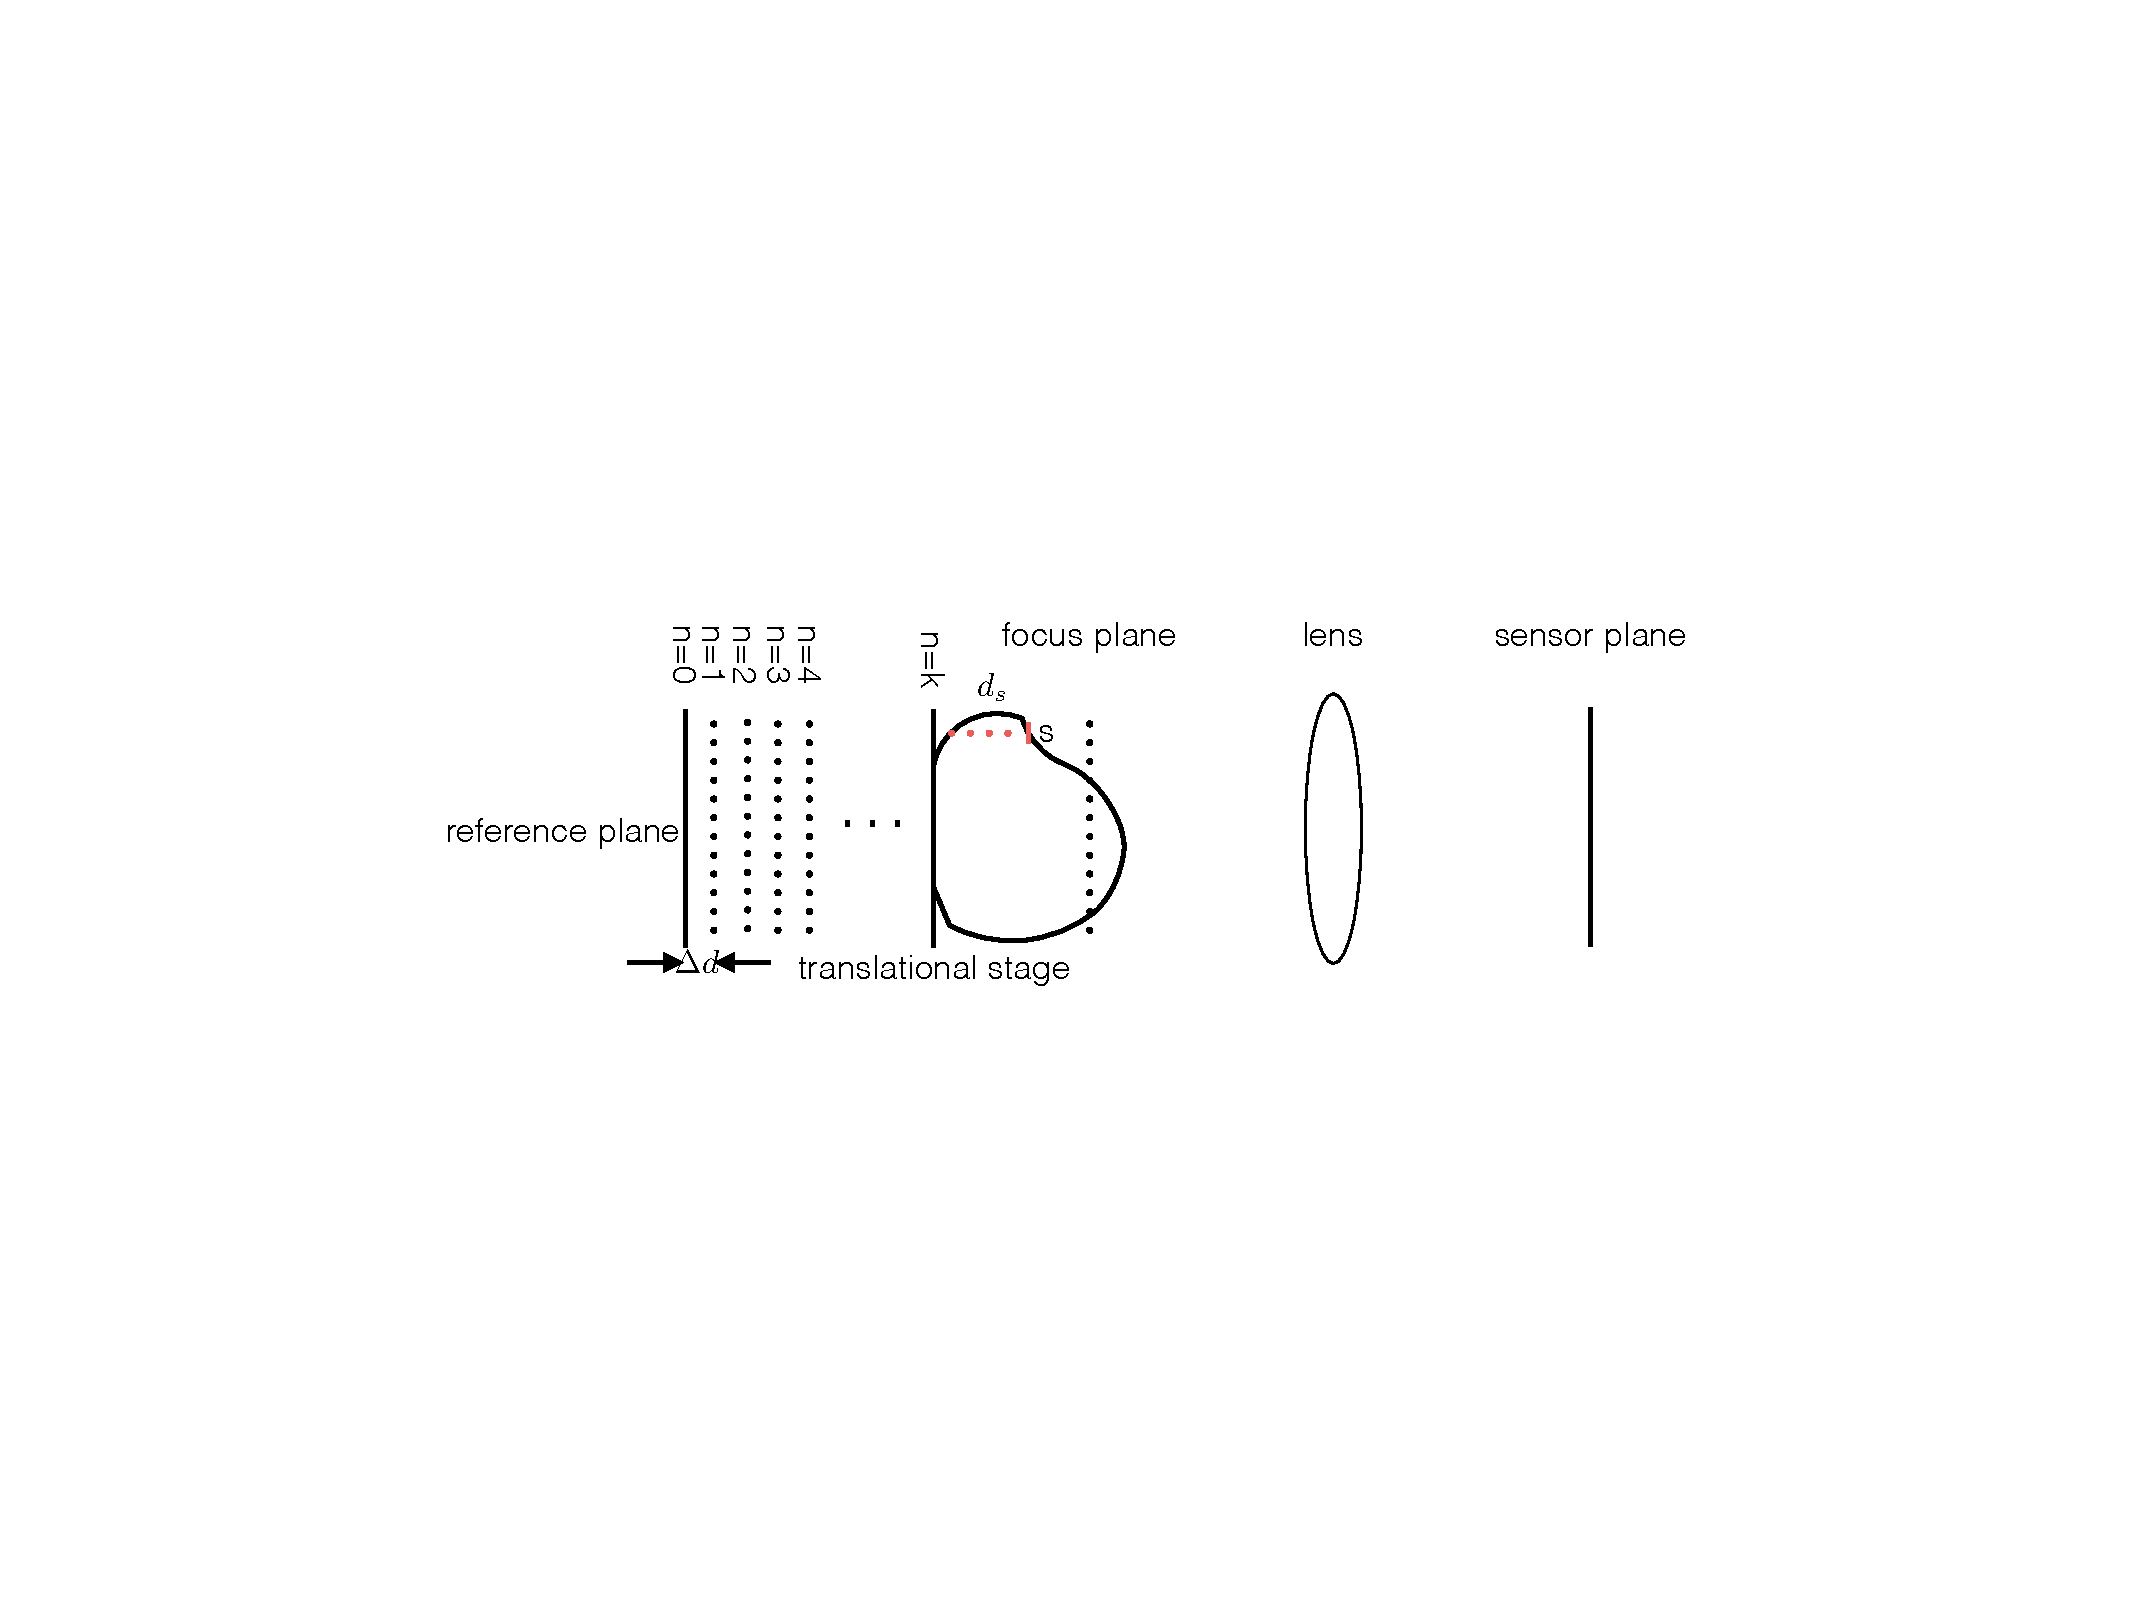
\includegraphics[width=0.8\textwidth]{relatedwork/shape_from_focus}
% \caption{shape from focus}
% \label{fig:shape_from_focus}
% \end{figure}
